\documentclass{article}
\usepackage[utf8]{inputenc} %кодировка
\usepackage[T2A]{fontenc}
\usepackage[english,russian]{babel} %русификатор 
\usepackage{mathtools} %библиотека матеши
\usepackage[left=1cm,right=1cm,top=2cm,bottom=2cm,bindingoffset=0cm]{geometry} %изменение отступов на листе
\usepackage{amsmath}
\usepackage{graphicx} %библиотека для графики и картинок
\graphicspath{}
\DeclareGraphicsExtensions{.pdf,.png,.jpg,.svg}
\usepackage{subcaption}
\usepackage{pgfplots}
\usepackage{float}
\usepackage{multirow}
\usepackage{listings}
\usepackage{xcolor}
\usepackage{tikz}
\usetikzlibrary{automata,positioning}
\usepackage{graphicx}
\usepackage{svg}  % Add this line



\lstset{
    backgroundcolor=\color{white},   % Цвет фона
    basicstyle=\footnotesize\ttfamily, % Шрифт
    breaklines=true,                  % Перенос строк
    frame=single,                     % Рамка вокруг кода
}


\begin{document}
% НАЧАЛО ТИТУЛЬНОГО ЛИСТА
\begin{center}
    \Large
    Федеральное государственное автономное \\
    образовательное учреждение высшего образования \\ 
    «Научно-образовательная корпорация ИТМО»\\
    \vspace{0.5cm}
    \large
    Факультет программной инженерии и компьютерной техники \\
    Направление подготовки 09.03.04 Программная инженерия \\
    \vspace{1cm}
    \Large
    \textbf{Отчёт по лабораторной работе № 2} \\
    По дисциплине «Моделирование» (семестр 5)\\
    \large
    \vspace{8cm}

    \begin{minipage}{.33\textwidth}
    \end{minipage}
    \hfill
    \begin{minipage}{.4\textwidth}
    
        \textbf{Студенты}: \vspace{.1cm} \\
        \ Дениченко Александр P3312\\
        \ Балин Артём P3312\\
        \ Кобелев Роман P3312\\
        \textbf{Практик}:  \\
        \ Мартынчук Илья Геннадьевич
    \end{minipage}
    \vfill
Санкт-Петербург\\ 2024 г.
\end{center}
\pagestyle{empty}
% КОНЕЦ ТИТУЛЬНОГО ЛИСТА 
\newpage
\pagestyle{plain}

\section*{Цель работы}
Изучение метода марковских случайных процессов и его применение для
исследования простейших моделей – систем массового обслуживания (СМО) с
однородным потоком заявок.

\section{Исходные данные}
Система 1: 

- Кол-во приборов: 2

- Ёмкость накопителей: 2/1 (для первого/второго приборов)
\\ \\
Система 2: 

- Кол-во приборов: 1

- Закон распределения длительности обслуживания: гиперэкспоненциальный с коэф-том вариации v = 1.5

- Ёмкость накопителя: 2
\\ \\
Критерий эффективности: минимальные потери заявок
\\ \\
Параметры загрузки (12 группа):

- интенсивнось потока: $\lambda = 0.7 \ c^{-1}$

- средняя длительность обслуживания: $b = 5\ c$

- вероятность занятия первого прибора: $p_1 = 0.8$

- вероятность занятия второго прибора: $p_2 = 0.2$
\\ \\
Интенсивность обслуживания: $\mu = \frac{1}{b} = 0.2 \ c^{-1}$
\\ \\
\section{Выполнение}
\subsection*{Состояния системы 1}

\begin{table}[h]
    \centering
    \begin{tabular}{|c|c|c|}
    \hline
    Комбинация & Обозначение & Вероятность \\
    \hline
    0/0/0/0 & $S_1$ &  0.013593\\
    1/0/0/0 & $S_2$ &  0.038061\\
    1/0/1/0 & $S_3$ &  0.106570\\
    1/0/2/0 & $S_4$ &  0.298397\\
    0/1/0/0 & $S_5$ &  0.009515\\
    0/1/0/1 & $S_6$ &  0.006661\\
    1/1/0/0 & $S_7$ &  0.026643\\
    1/1/1/0 & $S_8$ &  0.074599\\
    1/1/2/0 & $S_9$ &  0.208878\\
    1/1/0/1 & $S_{10}$ &  0.018650\\
    1/1/1/1 & $S_{11}$ &  0.052219\\
    1/1/2/1 & $S_{12}$ &  0.146214\\
    \hline
    \end{tabular}
    \caption{Система 1}
    \label{tab:system1}
\end{table}
Результат: Сумма вероятностей: 1.000000
\subsection*{Граф переходов системы 1}
\begin{center}
    \begin{tikzpicture}[
        ->,
        >=stealth,
        node distance=3cm,
        every state/.style={thick, fill=white},
        transform shape  % Масштабирует также текст и узлы
    ]
    \node[state] (S1) {$S_1$};
    \node[state] (S2) [right of=S1] {$S_2$};
    \node[state] (S3) [right of=S2] {$S_3$};
    \node[state] (S4) [right of=S3] {$S_4$};
    \node[state] (S5) [below of=S1] {$S_5$};
    \node[state] (S7) [right of=S5] {$S_7$};
    \node[state] (S8) [right of=S7] {$S_8$};
    \node[state] (S9) [right of=S8] {$S_9$};
    \node[state] (S6) [below of=S5] {$S_6$};
    \node[state] (S10) [right of=S6] {$S_{10}$};
    \node[state] (S11) [right of=S10] {$S_{11}$};
    \node[state] (S12) [right of=S11] {$S_{12}$};

        % 1
        \path (S1) edge[bend left] node[above] {$p_1\lambda$} (S2)
            (S2) edge[bend left] node[above] {$\mu$} (S1);

        \path (S5) edge[bend left] node[right] {$\mu$} (S1)
            (S1) edge[bend left] node[right] {$p_2\lambda$} (S5);
        
        % 2
        \path (S2) edge[bend left] node[above] {$p_1\lambda$} (S3)
            (S3) edge[bend left] node[above] {$\mu$} (S2);

        \path (S2) edge[bend left] node[right] {$p_2\lambda$} (S7)
            (S7) edge[bend left] node[right] {$\mu$} (S2);

        % 3
        \path (S3) edge[bend left] node[above] {$p_1\lambda$} (S4)
            (S4) edge[bend left] node[above] {$\mu$} (S3);

        \path (S3) edge[bend left] node[right] {$p_2\lambda$} (S8)
            (S8) edge[bend left] node[right] {$\mu$} (S3);

        % 4
        \path (S4) edge[bend left] node[right] {$p_2\lambda$} (S9)
            (S9) edge[bend left] node[right] {$\mu$} (S4);

        % 5
        \path (S5) edge[bend left] node[below] {$p_1\lambda$} (S7)
            (S7) edge[bend left] node[below] {$\mu$} (S5);

        \path (S5) edge[bend left] node[left] {$p_2\lambda$} (S6)
            (S6) edge[bend left] node[left] {$\mu$} (S5);

        % 6
        \path (S6) edge[bend left] node[below] {$p_1\lambda$} (S10)
            (S10) edge[bend left] node[below] {$\mu$} (S6);

        % 7
        \path (S7) edge[bend left] node[below] {$p_1\lambda$} (S8)
            (S8) edge[bend left] node[below] {$\mu$} (S7);

        \path (S7) edge[bend left] node[left] {$p_2\lambda$} (S10)
            (S10) edge[bend left] node[left] {$\mu$} (S7); 
        
        % 8
        \path (S8) edge[bend left] node[below] {$p_1\lambda$} (S9)
            (S9) edge[bend left] node[below] {$\mu$} (S8);

        \path (S8) edge[bend left] node[left] {$p_2\lambda$} (S11)
            (S11) edge[bend left] node[left] {$\mu$} (S8); 

        % 9
        \path (S9) edge[bend left] node[left] {$p_2\lambda$} (S12)
            (S12) edge[bend left] node[left] {$\mu$} (S9);

        % 10
        \path (S10) edge[bend left] node[below] {$p_1\lambda$} (S11)
            (S11) edge[bend left] node[below] {$\mu$} (S10);

        % 11
        \path (S11) edge[bend left] node[below] {$p_1\lambda$} (S12)
            (S12) edge[bend left] node[below] {$\mu$} (S11);


    \end{tikzpicture}
\end{center}
\subsection*{Матрица интенсивностей переходов системы 1}

\begin{table}[H]
    \centering
    \begin{tabular}{c|rrrrrrrrrrrr}
        & $S_1$ & $S_2$ & $S_3$ & $S_4$ & $S_5$ & $S_6$ & $S_7$ & $S_8$ & $S_9$ & $S_{10}$ & $S_{11}$ & $S_{12}$ \\
        \hline
        $S_1$     & -0.70 & 0.56 & 0.00 & 0.00 & 0.14 & 0.00 & 0.00 & 0.00 & 0.00 & 0.00 & 0.00 & 0.00 \\
        $S_2$     & 0.20 & -0.90 & 0.56 & 0.00 & 0.00 & 0.00 & 0.14 & 0.00 & 0.00 & 0.00 & 0.00 & 0.00 \\
        $S_3$     & 0.00 & 0.20 & -0.90 & 0.56 & 0.00 & 0.00 & 0.00 & 0.14 & 0.00 & 0.00 & 0.00 & 0.00 \\
        $S_4$     & 0.00 & 0.00 & 0.20 & -0.34 & 0.00 & 0.00 & 0.00 & 0.00 & 0.14 & 0.00 & 0.00 & 0.00 \\
        $S_5$     & 0.20 & 0.00 & 0.00 & 0.00 & -0.90 & 0.14 & 0.56 & 0.00 & 0.00 & 0.00 & 0.00 & 0.00 \\
        $S_6$     & 0.00 & 0.00 & 0.00 & 0.00 & 0.20 & -0.76 & 0.00 & 0.00 & 0.00 & 0.56 & 0.00 & 0.00 \\
        $S_7$     & 0.00 & 0.20 & 0.00 & 0.00 & 0.20 & 0.00 & -1.10 & 0.56 & 0.00 & 0.14 & 0.00 & 0.00 \\
        $S_8$     & 0.00 & 0.00 & 0.20 & 0.00 & 0.00 & 0.00 & 0.20 & -1.10 & 0.56 & 0.00 & 0.14 & 0.00 \\
        $S_9$     & 0.00 & 0.00 & 0.00 & 0.20 & 0.00 & 0.00 & 0.00 & 0.20 & -0.54 & 0.00 & 0.00 & 0.14 \\
        $S_{10}$  & 0.00 & 0.00 & 0.00 & 0.00 & 0.00 & 0.20 & 0.20 & 0.00 & 0.00 & -0.96 & 0.56 & 0.00 \\
        $S_{11}$  & 0.00 & 0.00 & 0.00 & 0.00 & 0.00 & 0.00 & 0.00 & 0.20 & 0.00 & 0.20 & -0.96 & 0.56 \\
        $S_{12}$  & 0.00 & 0.00 & 0.00 & 0.00 & 0.00 & 0.00 & 0.00 & 0.00 & 0.20 & 0.00 & 0.20 & -0.40
    \end{tabular}
    \caption{Матрица интенсивностей переходов}
    \label{tab:intensity_matrix}
\end{table}

\subsection*{Характеристика системы 1}

\begin{table}[H]
    \centering
    \begin{tabular}{|l|l|r|l|}
    \hline
    Характеристика & Прибор & Значение & Формула расчета \\
    \hline
    \multirow{3}{*}{Нагрузка} 
    & П1 & 2.8000 & $\rho_1 = \frac{\lambda p_1}{\mu} = \frac{0.7 \cdot 0.8}{5} \cdot 20 = 2.8$ \\
    & П2 & 0.7000 & $\rho_2 = \frac{\lambda p_2}{\mu} = \frac{0.7 \cdot 0.2}{5} \cdot 20 = 0.7$ \\
    & Сумм & 3.5000 & $\rho = \rho_1 + \rho_2$ \\
    \hline
    \multirow{3}{*}{Загрузка} 
    & П1 & 0.9702 & $Y_1 = 1 - P_1 - P_5 - P_6$ \\
    & П2 & 0.5434 & $Y_2 = 1 - P_1 - P_2 - P_3 - P_4$ \\
    & Сред & 0.7568 & $Y_{ср} = \frac{Y_1 + Y_2}{2}$ \\
    \hline
    \multirow{3}{*}{Длина очереди} 
    & П1 & 1.5404 & $L_1 = (P_3 + P_8 + P_{11}) + 2(P_4 + P_9 + P_{12})$ \\
    & П2 & 0.2237 & $L_2 = P_6 + P_{10} + P_{11} + P_{12}$ \\
    & Сумм & 1.7641 & $L = L_1 + L_2$ \\
    \hline
    \multirow{3}{*}{Число заявок} 
    & П1 & 2.5106 & $M_1 = L_1 + Y_1$ \\
    & П2 & 0.7671 & $M_2 = L_2 + Y_2$ \\
    & Сумм & 3.2777 & $M = M_1 + M_2$ \\
    \hline
    \multirow{3}{*}{Время ожидания} 
    & П1 & 2.7507 & $W_1 = \frac{L_1}{\lambda p_1}$ \\
    & П2 & 1.5981 & $W_2 = \frac{L_2}{\lambda p_2}$ \\
    & Сумм & 2.5202 & $W = \frac{L}{\lambda}$ \\
    \hline
    \multirow{3}{*}{Время пребывания} 
    & П1 & 7.7507 & $U_1 = W_1 + \frac{1}{\mu}$ \\
    & П2 & 6.5981 & $U_2 = W_2 + \frac{1}{\mu}$ \\
    & Сумм & 14.3488 & $U = U_1 + U_2$ \\
    \hline
    \multirow{3}{*}{Вероятность потери} 
    & П1 & 0.3660 & $e_{1} = (P_4 + P_{9} + P_{12}) \cdot p_1$ \\
    & П2 & 0.0313 & $e_{2} = (P_{6} + P_{10} + P_{11} + P_{12}) \cdot p_2$ \\
    & Сумм & 0.3973 & $e_{} = e_{1} + e_{2}$ \\
    \hline
    \multirow{3}{*}{Производительность} 
    & П1 & 0.3551 & $A_1 = \lambda p_1(1 - e_{1})$ \\
    & П2 & 0.1356 & $A_2 = \lambda p_2(1 - e_{2})$ \\
    & Сумм & 0.4907 & $A = A_1 + A_2$ \\
    \hline
    \end{tabular}
    \caption{Характеристики системы массового обслуживания с формулами расчета}
    \label{tab:queueing_system}
\end{table}




\subsection*{Состояния системы 2}

\begin{table}[h]
    \centering
    \begin{tabular}{|c|c|c|}
    \hline
    Комбинация & Обозначение & Вероятность \\
    \hline
    0/0 & $S_1$ & 0.0347 \\
    1(1)/0 & $S_2$ & 0.0380 \\
    1(2)/0 & $S_3$ & 0.0362 \\
    1(1)/1 & $S_4$ & 0.0915 \\
    1(2)/1 & $S_5$ & 0.0755 \\
    1(1)/2 & $S_6$ & 0.0304 \\
    1(2)/2 & $S_7$ & 0.0937 \\
    \hline
    \end{tabular}
    \caption{Система 2}
    \label{tab:system2}
\end{table}
\subsection*{Граф переходов системы 2}


\begin{figure}[H]
    \centering
    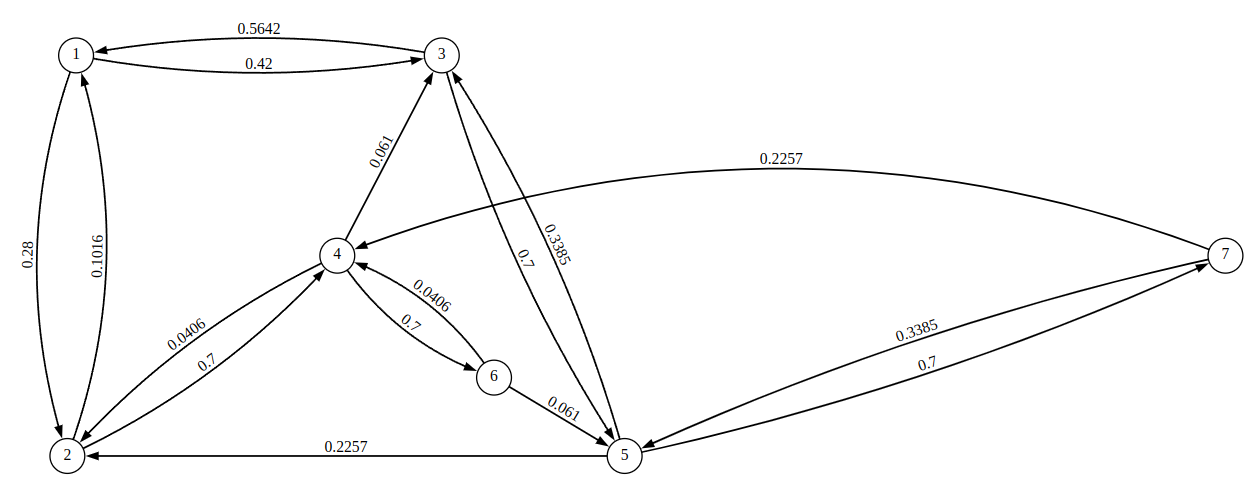
\includegraphics[width=.9\textwidth]{image.png}
    \caption{Граф переходов системы 2}
    \label{fig:system2-graph}
\end{figure}

\subsection*{Матрица интенсивностей переходов системы 2}
\begin{table}[H]
    \centering
    \begin{tabular}{c|rrrrrrr}
        & 1 & 2 & 3 & 4 & 5 & 6 & 7 \\
        \hline
        1 & -0.7000 & 0.2800 & -0.4200 & 0.7000 & 0.0000 & 0.0000 & 0.0000 \\
        2 & 0.1016 & -0.8016 & 0.0000 & 0.0000 & 0.0000 & 0.0000 & 0.0000 \\
        3 & 0.5642 & 0.0000 & -1.2642 & 0.0000 & 0.7000 & 0.0000 & 0.0000 \\
        4 & 0.0000 & 0.0406 & 0.0610 & -0.8016 & 0.0000 & 0.7000 & 0.0000 \\
        5 & 0.0000 & 0.2257 & 0.3385 & 0.0000 & -1.2642 & 0.0000 & 0.7000 \\
        6 & 0.0000 & 0.0000 & 0.0000 & 0.0406 & 0.0610 & -0.1016 & 0.0000 \\
        7 & 0.0000 & 0.0000 & 0.0000 & 0.2257 & 0.3385 & 0.0000 & -0.5642
    \end{tabular}
    \caption{Матрица интенсивностей переходов системы 2}
    \label{tab:intensity_matrix_2}
\end{table}

\subsection*{Характеристика системы 2}

\begin{table}[H]
    \centering
    \begin{tabular}{|l|l|r|l|}
    \hline
    Характеристика & Прибор & Значение & Формула расчета \\
    \hline
    Нагрузка & П1 & 3.5000 & $\rho = \lambda b$ \\
    \hline
    Загрузка & П1 & 0.9653 & $Y = 1 - P_1$ \\
    \hline
    Длина очереди & П1 & 1.6152 & $L = (P_4 + P_5) + 2(P_6 + P_7)$ \\
    \hline
    Число заявок & П1 & 2.5805 & $M = L + Y$ \\
    \hline
    Время ожидания & П1 & 2.3074 & $W = \frac{L}{\lambda}$ \\
    \hline
    Время пребывания & П1 & 7.3074 & $U = W + q\cdot t_1 + (1 - q)\cdot t_2$ \\
    \hline
    Вероятность потери & П1 & 0.5069 & $e = \lambda \cdot (P_6 + P_7)$ \\
    \hline
    Производительность & П1 & 0.3452 & $A = \lambda \cdot (1 - e)$ \\
    \hline
    \end{tabular}
    \caption{Характеристики системы массового обслуживания}
    \label{tab:queueing_system_characteristics}
\end{table}
\[t_1  = \left(1 + \sqrt{\frac{1-q}{2q}(v^2-1)}\right) \cdot b = 9.8412\]  \[t_2 = \left(1 - \sqrt{\frac{q}{2(1-q)}(v^2-1)}\right) \cdot b = 1.7725\] - времена обслуживания 
для двух разных путей (при гиперэкспоненциальном распределении), где $q = 0.4$ - вероятность выбора первого пути, $v = 1.5$ - параметр, характеризующий степень гиперэкспоненциальности.
\section{Сравнение систем}

\begin{table}[H]
    \centering
    \begin{tabular}{|l|r|r|r|}
    \hline
    Характеристика & Система 1 & Система 2 & Разница (\%) \\
    \hline
    Нагрузка & 3.5000 & 3.5000 & 0.00 \\
    Загрузка & 0.7568 & 0.9653 & 21.60 \\
    Длина очереди & 1.7641 & 1.6152 & 8.44 \\
    Число заявок & 3.2777 & 2.5805 & 21.27 \\
    Время ожидания & 2.5202 & 2.3074 & 8.44 \\
    Время пребывания & 14.3488 & 7.3074 & 49.07 \\
    Вероятность потери & 0.3973 & 0.5069 & 21.62 \\
    Производительность & 0.4219 & 0.3452 & 18.18 \\
    \hline
    \end{tabular}
    \caption{Сравнение характеристик систем}
    \label{tab:system_comparison}
\end{table}

\begin{figure}[H]
    \centering
    \begin{tikzpicture}
    \begin{axis}[
        width=12cm,
        height=8cm,
        ybar,
        bar width=15pt,
        ylabel={Значение},
        xlabel={},
        symbolic x coords={Загрузка, Длина очереди, Число заявок, Время ожидания, Время пребывания, Вер. потери, Производит.},
        xtick=data,
        xticklabel style={rotate=45, anchor=east},
        legend style={at={(0.5,1.05)}, anchor=south},
        legend columns=2,
        ymin=0
    ]
    \addplot coordinates {
        (Загрузка,0.7568)
        (Длина очереди,1.7641)
        (Число заявок,3.2777)
        (Время ожидания,2.5202)
        (Время пребывания,14.3488)
        (Вер. потери,0.3973)
        (Производит.,0.4219)
    };
    \addplot coordinates {
        (Загрузка,0.9653)
        (Длина очереди,1.6152)
        (Число заявок,2.5805)
        (Время ожидания,2.3074)
        (Время пребывания,7.3074)
        (Вер. потери,0.5069)
        (Производит.,0.3452)
    };
    \legend{Система 1, Система 2}
    \end{axis}
    \end{tikzpicture}
    \caption{Сравнение характеристик систем}
    \label{fig:system_comparison}
\end{figure}
Нагрузка не включена в график, так как она одинакова для обеих систем (3.5).
\section*{Вывод }
На основе сравнительного анализа характеристик функционирования двух систем массового обслуживания можно сделать следующие выводы:

1. При одинаковой нагрузке (3.5) система 2 показывает более высокую загрузку (0.9653 против 0.7568), что говорит о более эффективном использовании ресурсов прибора.

2. Система 1 демонстрирует более высокие показатели:

   - длины очереди (1.7641 против 1.6152)

   - числа заявок в системе (3.2777 против 2.5805)
   
   - времени пребывания заявок (14.3488 против 7.3074)
   
3. Система 2, несмотря на более простую структуру (один прибор), имеет более высокую вероятность потери заявок (0.5069 против 0.3973), что является её основным недостатком.

4. По критерию \textbf{минимальных потерь} заявок система 1 (двухканальная) оказывается более эффективной, так как имеет меньшую вероятность потери заявок и более высокую производительность (0.4219 против 0.3452).



\end{document}
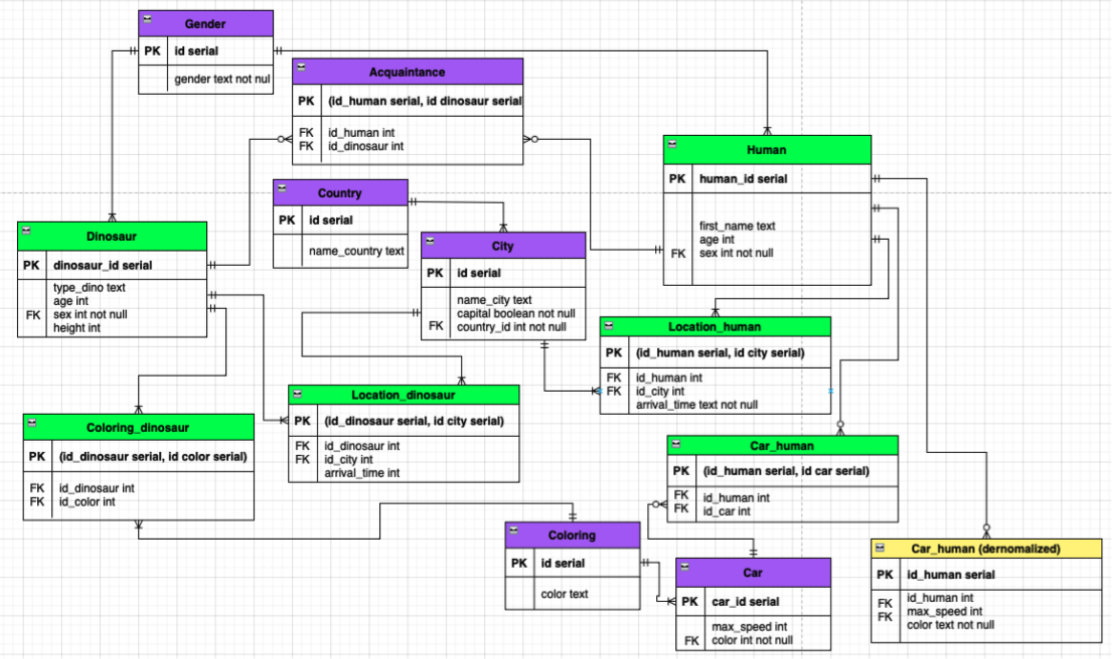
\includegraphics[width=.9\textwidth]{123}



